
%% \gad Macros to refer to snapshot's pointers and line-numbers are
%% defined together with the Figure in

%\newcommand{\fx}{\text{fx}}
%\newcommand{\fy}{\text{fy}}
%\newcommand{\x}{\text{x}}
%\newcommand{\y}{\text{y}}
%\newcommand{\s}{\text{S}}

\newcommand{\fx}{\mathit{fx}}
\newcommand{\fy}{\mathit{fy}}
\newcommand{\x}{x}
\newcommand{\y}{y}
\newcommand{\s}{S}

%%\begin{wrapfigure}[9]{r}[0pt]{0.4\textwidth} 
%% \begin{figure}
%% %
%% \centering
%% \begin{tabular}{l l l}
%% %
%% %  
%% \begin{minipage}[l]{.30\textwidth}
%% \begin{alltt}
%% \num{1}  write (p, v): () \{
%% \num{2}    \act{write} (p, v);
%% \num{3}    b <- \act{read} (S);
%% \num{4}    \textbf{if} b 
%% \num{5}    \textbfthen \act{transfer} (p, v);
%% \num{6}    \textbf{else skip};\}
%% \end{alltt} 
%% \end{minipage}
%% %
%% & \hfill
%% %
%% \begin{minipage}[l]{.6\textwidth}
%% \begin{alltt}
%% \num{1}  scan (): \(A {\times} A\)  \{
%% \num{2}    \act{write} (S, true);
%% \num{3}    \act{write} (fx,\( \bot\));
%% \num{4}    \act{write} (fy,\( \bot\));
%% \num{5}    vx <- \act{read} (x);
%% \num{6}    vy <- \act{read} (y);
%% \num{7}    \act{write}(S, false);
%% \num{8}    ox <- \act{read} (fx);
%% \num{9}    oy <- \act{read} (fy);
%% \num{10}   \textbf{let} rx = \textbf{if} ox \(\neq \bot\) \textbfthen ox \textbf{else} vx;  
%% \num{11}   \textbf{let} ry = \textbf{if} oy \(\neq \bot\) \textbfthen oy \textbf{else} vy;  
%% \num{11}   \act{relink}(rx, ry);
%% \num{12}   \textbf{return} (rx, ry);
%% \end{alltt} 
%% \end{minipage}
%% %
%% \end{tabular}
%% %
%% \caption{Jayanti's single-scanner, single-writer snapshot algorithm}
%% \label{fig:jayanti}
%% \end{figure}
%\end{wrapfigure}

\newcommand{\actwrite}[2]{{#1}\,{:=}\,{#2}}

% The following version saves a little more space
\begin{figure}
%
\centering
\begin{tabular}{c@{\ \ \ \ \ }c}
%  
\begin{minipage}[t][3.7cm][t]{.5\textwidth}
\small
\begin{alltt}
\num{1} write (p : ptr, v : \(A\)) \{
\num{2}  \actwrite{p}{v};
\num{3}  b \tbnd \act{read}(S);
\num{4}  if b 
\num{5}  then \actwrite{(f_of p)}{v}
\num{6}  {else return} \}

  f_of (p : ptr) \{
   return p = x ? fx : fy \}
\end{alltt}
\end{minipage}
%
&
\begin{minipage}[t][3.7cm][t]{.5\textwidth}
\small
\begin{alltt}
\num{ 7} scan (): \(A {\times} A\)  \{
\num{ 8}  \actwrite{S}{true};
\num{ 9}  \actwrite{fx}{\(\bot\)}; \actwrite{fy}{\(\bot\)};
\num{10}  vx \tbnd \act{read}(x); vy \tbnd \act{read}(y);
\num{11}  \actwrite{S}{false};
\num{12}  ox \tbnd \act{read}(fx); oy \tbnd \act{read}(fy);
\num{13}  rx \tbnd if (ox \(\neq\bot\)) then ox {else} vx;  
\num{14}  ry \tbnd if (oy \(\neq\bot\)) then oy {else} vy;  
\num{15}  return (rx, ry) \}
\end{alltt} 
\end{minipage}
%
\end{tabular}
%
\caption{Jayanti's single-scanner/single-writer snapshot algorithm.}
\label{fig:jayanti-snapshot}
\end{figure}



\newcommand{\jywrite}{\texttt{write}\xspace}
\newcommand{\jyscan}{\texttt{scan}\xspace}

\section{Verification challenge and main ideas}
\label{sc:overview}


Jayanti's snapshot algorithm~\cite{Jayanti+STOC05} provides the
functionality of a shared array of size $m$, operated on by two
procedures: \jywrite, which stores a given value into an element, and
\jyscan, which returns the array's contents. We use the
\emph{single-writer}/\emph{single-scanner} version of the algorithm.
which assumes that at most one thread writes into an element, and at
most one thread invokes the scanner, at any given time. In other
words, there is a scanner lock and $m$ per-element locks. A thread
that wants to scan, has to acquire the scanner lock first, and a
thread that wants to write into element $i$ has to acquire the $i$-th
element lock. However, scanning and writing into different elements
can proceed concurrently.
% 
%where a thread acquires a writer lock for a particular element before
%writing into it, and a scanner before scanning. A scanner lock does
%not preclude writing, and a writer lock for an element does not
%preclude scanning, or writing into other elements. 
This is the simplest of Jayanti's algorithms, but it already exhibits
linearization points of dynamic nature. We also restrict the array
size to $m\,{=}\,2$ (\ie, we consider two pointers $\x$ and $\y$,
instead of an array). This removes some tedium from verification, but
exhibits the same conceptual challenges.
 
The difficulty in this snapshot algorithm is ensuring that the scanner
returns the most recent snapshot of the memory. A na\"{i}ve scanner, which
simply reads $\x$ and $\y$ in succession, is unsound. To see why,
consider the following scenario, starting with $\x=5$, $\y=0$. The
scanner reads $\x$, but before it reads $\y$, another thread preempts
it, and changes $\x$ to $2$ and, subsequently, $\y$ to $1$. The
scanner continues to read $\y$, and returns $\x=5, \y=1$, which was
never the contents of the memory. Moreover, $(\x, \y)$, changed from
$(5,0)$ to $(2, 0)$ to $(2, 1)$ as a result of distinct
non-overlapping writes; thus, it is impossible to find a linearization
point for the scan because linearizability only permits reordering of
overlapping operations.

%\ab{Remove rest?} by dynamically reordering non-overlapping
%operations, as permitted by linearizability (though we show further
%below a scenario when {\jyscan} is justified in returning a pair that
%was not the contents of the memory).

%\gad{Do we make the latter example a graph/ figure somehow? We have
%  done so for the slides}

To ensure a sound snapshot, Jayanti's algorithm internally keeps
additional \emph{forwarding pointers} $\fx$ and $\fy$, and a boolean
\emph{scanner bit} $\s$. The implementation is given in
Figure~\ref{fig:jayanti-snapshot}.\footnote{Following Jayanti, we
  simplify the presentation and omit the locking code that ensures the
  single-writer/single-scanner setup. Of course, in our Coq
  development~\cite{CoqFiles}, we make the locking explicit.}
%
The intuition is as follows. A writer storing $v$ into $p$
(line~\lineWrtWrt), will additionally store $v$ into the forwarding
pointer for $p$ (line~\lineWrtFwd), provided $S$ is set. If the
scanner missed the write and instead read the old value of $p$
(lines~\lineScanReadsX--\lineScanReadsY), it will have a chance to
catch $v$ via the forwarding pointer
(lines~\lineScanReadsFX--\lineScanReadsFY). The scanner bit $S$ is
used by writers (line~\lineWrtChk) to detect a scan in progress, and
forward $v$.

{
%\setlength{\belowcaptionskip}{-5pt} 
\begin{figure}[t]
%
\captionsetup[subfigure]{justification=centering}
\centering  
\begin{subfigure}[t]{1\textwidth}
\centering
\begin{tabular}{l || l || l}
  \texttt{l: }\texttt{write (x,2);}\quad &
   \multirow{2}{*}{\texttt{c: scan ()}}\quad & 
    \multirow{2}{*}{\texttt{r: write (x,3)}}  \\
  \phantom{\texttt{l: }}\texttt{write (y,1)} & &   
\end{tabular}
\caption{\label{fig:weird:code}Parallel composition of three threads \texttt{l, c, r}.}
\end{subfigure}\\

\begin{subfigure}[b]{1\textwidth}
\begin{tabular}{l@{\hfill} l@{\hfil}}
\begin{minipage}[t]{0.5\textwidth}
\begin{alltt}
 \num{1}  c: \actwrite{S}{true}
 \num{2}  c: \actwrite{fx}{\(\bot\)}
 \num{3}  c: \actwrite{fy}{\(\bot\)}
 \num{4}  c: \act{read}(x)  // vx <- 5
 \num{5}  c: \act{read}(y)  // vy <- 0
 \num{6}  l: \actwrite{x}{2}
 \num{7}  l: \act{read}(S)  // b <- true
 \num{8}  l: \actwrite{fx}{2} 
 \num{9}  l: return ()
\num{10}  r: \actwrite{x}{3}
\end{alltt}
\end{minipage}
&
\begin{minipage}[t]{0.33\textwidth}
\begin{alltt}
\num{11} l: \actwrite{y}{1}
\num{12} l: \act{read}(S)  // b <- true
\num{13} l: \actwrite{fy}{1}
\num{14} l: return ()
\num{15} c: \actwrite{S}{false}
\num{16} r: \act{read}(S)  // b <- false
\num{17} r: return ()
\num{18} c: \act{read}(fx) // ox <- 2
\num{19} c: \act{read}(fy) // oy <- 1
\num{20} c: return (2,1)
\end{alltt} 
\end{minipage}
%
\end{tabular}
\caption{\label{fig:weird:exec} A possible interleaving of the threads
  in~(\subref{fig:weird:code}).}
\end{subfigure}
\caption{\label{fig:weird} An example leading to a scanner miss.%
}
\end{figure}
}

 
As Jayanti proves, this implementation \emph{is} linearizable. Informally,
every overlapping calls to \jywrite~and \jyscan~can be rearranged to
appear as if they occurred sequentially.  To illustrate, consider the
program in Figure~\ref{fig:weird:code}, and one possible interleaving
of its primitive memory operations in Figure~\ref{fig:weird:exec}. The
threads {\tt l}, {\tt c}, and {\tt r}, start with $\x = 5, \y = 0$.
%
The thread {\tt c} is scheduled first, and through lines~1--5 sets the
scanner bit, clears the forwarding pointers, and reads $\x = 5, \y =
0$. Then {\tt l} intervenes, and in lines~6--9, overwrites
$\x$ with $2$, and seeing $\s$ set, forwards $2$ to $\fx$. Next, {\tt
  r} and {\tt l} overlap, writing $3$ into $\x$ and $1$ into
$\y$. However, while $1$ gets forwarded to $\fy$ (line 13), $3$ is not
forwarded to $\fx$, because $\s$ was turned off in line 15 (\ie, the
scan is no longer in progress). Hence, when {\tt c} reads the
forwarded values (lines 18, 19), it returns $\x = 2, \y = 1$.

While $\x\,{=}\,2, \y\,{=}\,1$ was never the contents of the memory,
returning this snapshot is nevertheless justified because we can
\emph{pretend} that the scanner \emph{missed} {\tt r}'s write of
$3$. Specifically, the events in Figure~\ref{fig:weird:exec} can be
\emph{reordered} to represent the following sequential execution:
%
\begin{equation}
\hfill \mathtt{write\, (x, 2);\ write\, (y,1);\ scan\, ();\ write\, (x,
  3)}\hfill \label{eq:lin}
\end{equation}
%
Importantly, the client programs have no means to discover that a
different scheduling actually took place in real time, because they
can access the internal state of the algorithm only via interface
methods, \jywrite~and \jyscan.

This kind of temporal reordering is the most characteristic aspect of
linearizability proofs, which typically describe the reordering by
listing the linearization points of each procedure. At a linearization
point, the procedure's operations can be spliced into the execution
history as an uninterrupted chunk. For example, in Jayanti's proof,
the linearization point of \jyscan~is at line~\lineScanUnsetsS\ in
Figure~\ref{fig:jayanti-snapshot}, where the scanner bit is unset. The
linearization point of \jywrite, however, may vary. If
\jywrite~starts before an overlapping \jyscan's line~\lineScanUnsetsS,
and moreover, the \jyscan~misses the \jywrite---note the dynamic and
future-dependent nature of this property---, then \jywrite~should
appear after {\tt scan}; that is, the \jywrite's linearization point
is right after \jyscan's linearization point at line~\lineScanUnsetsS.
%
Otherwise, \jywrite's linearization point is at line~\lineWrtWrt.
%
In the former case, \jywrite~exactly has a non-local and
future-dependent linearization point, because the decision on the
logical order of this \jywrite~depends on the execution of \jyscan~in
a different thread. This decision takes effect on
lines~\lineScanReadsFX--\lineScanReadsFY, which can take place
\emph{after} the execution of \jywrite~has terminated.
%
For instance, in Figure~\ref{fig:weird:exec} the execution
of \jywrite~in \texttt{r} terminates at step 17, yet, in Jayanti's
proof, the decision to linearize this \jywrite\ after the
overlapping \jyscan\ is taken at line~18, when the \jyscan\ reads the
value from the previous \jywrite.

%%\gad{Rephrased the paragraph above to answer {\sf R1.Q5}}

%% \gad{Well, the non-regional argument is subtle and here is used with
%%   the wrong example: In this particular case, although the scanner bit
%%   is unset later at 15, the LP' of {\tt l} is fixed at line~11
%%   regardless of the future -- witnessed by the fact that it finishes
%%   green. The non-regionality argument has to be made about the
%%   position of the write to \x done by {\tt r}, which is the write that
%%   is relinked.}

%% \gad{When {\tt r} finishes in line~18, it's position in the final
%%   order is not settled as it depends on the scanners future: this
%%   write is missed by the scanner, and has to be relinked. This
%%   example, though showcases why relink is needed and how it works it
%%   does not showcase non-regionality: when 18 finishes, you have the
%%   information in lines 1-18 to determine that his position will be
%%   changed by scan before the end, so it can be linearized in line 18.}

\begin{figure}[t]
%\captionsetup[subfigure]{justification=centering}
\begin{subfigure}[t]{0.49\textwidth}
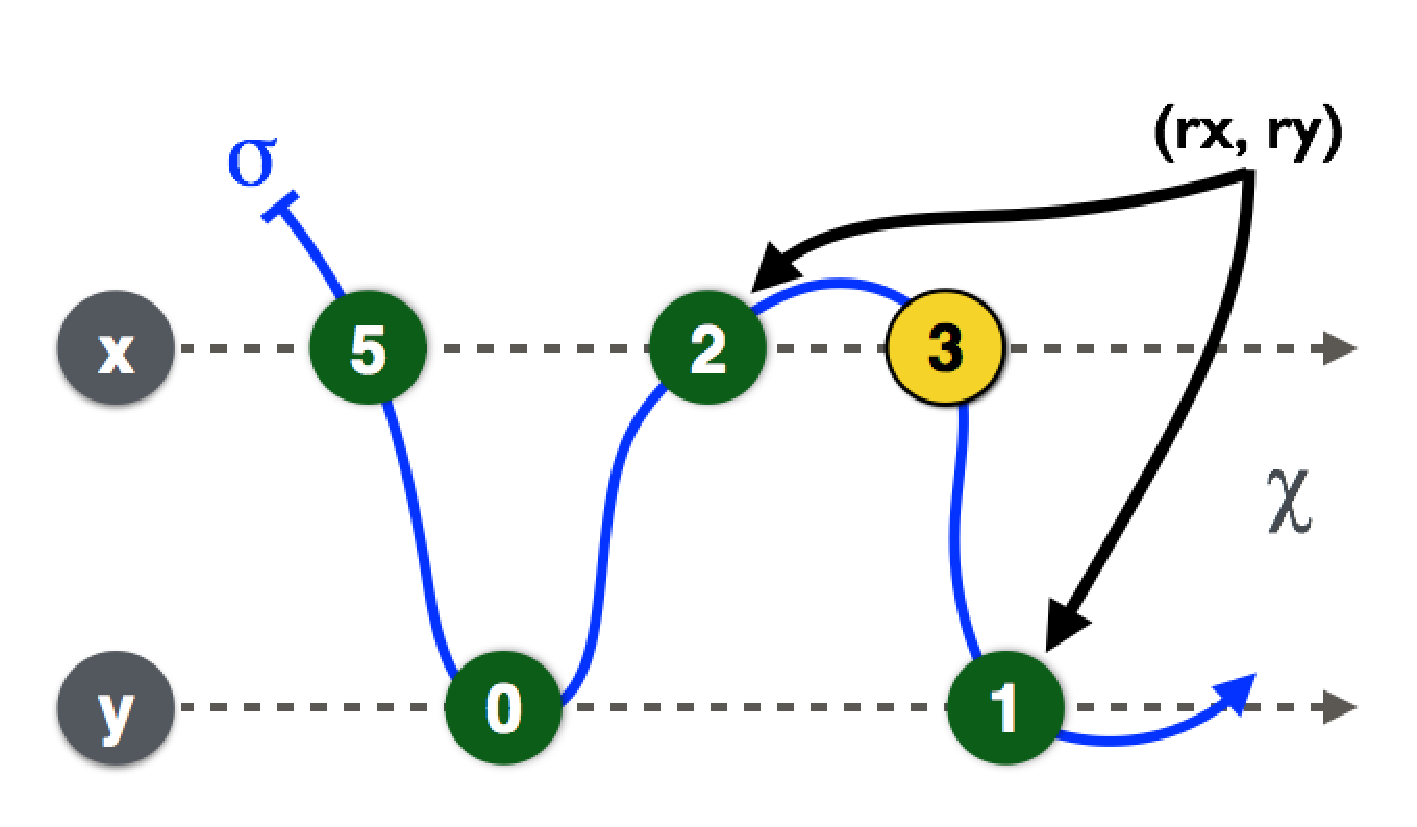
\includegraphics[width=6.1cm]{relink-before3.pdf}
\caption{\label{fig:reorder:before}} % Logical $=$ Real Time order, not a snapshot}
\end{subfigure} \hfill
\begin{subfigure}[t]{0.49\textwidth}
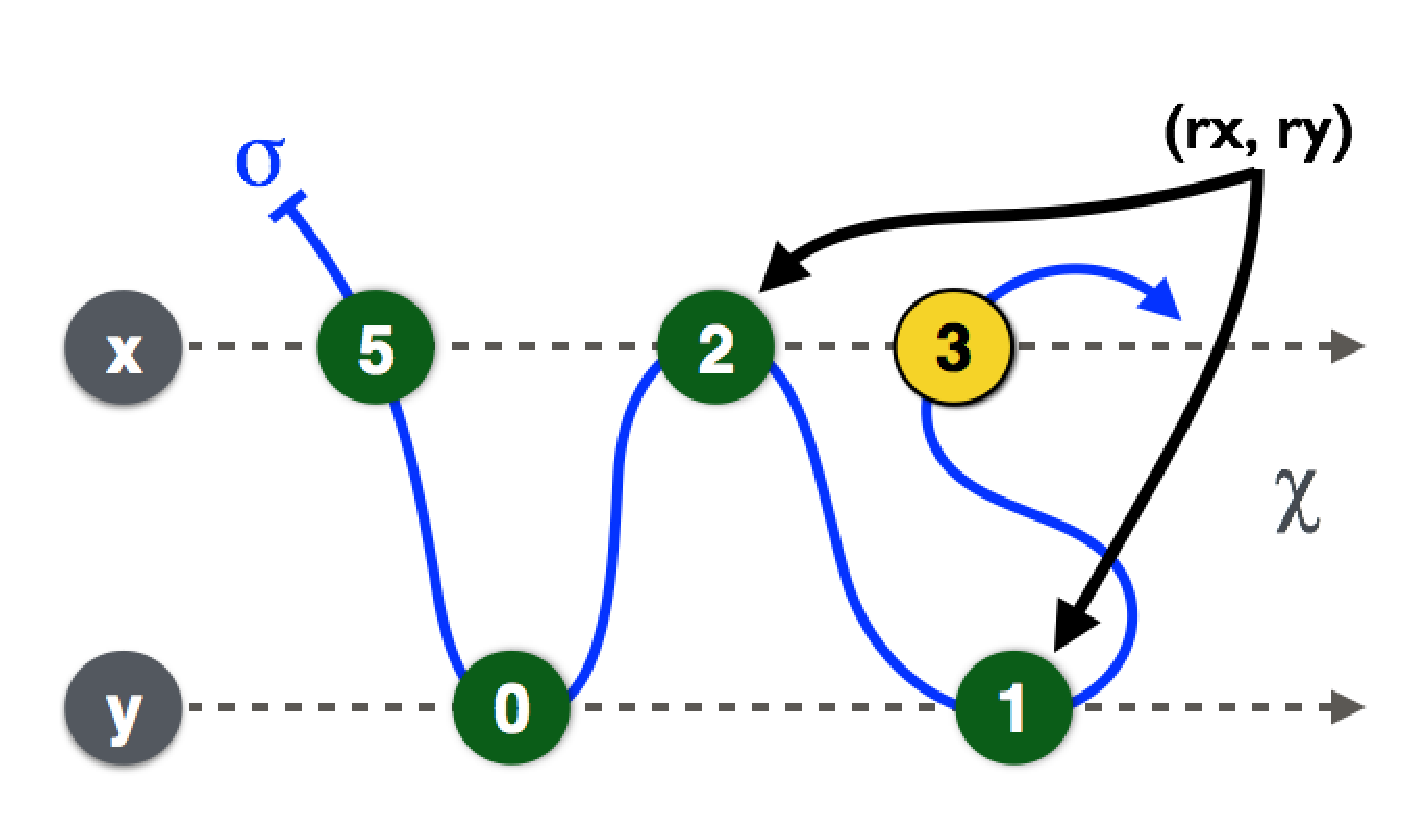
\includegraphics[width=6.1cm]{relink-after3.pdf}
\caption{\label{fig:reorder:after}} % Logical $\neq$ Real Time order, snapshot OK}
\end{subfigure}%
%
\caption{\label{fig:reorder} Changing the logical ordering (solid line
  $\ordlist$) of write events from (5, 0, 2, 3, 1) in
  (\subref{fig:reorder:before}) to (5, 0, 2, 1, 3) in
  (\subref{fig:reorder:after}), to reconcile with {\tt scan} returning
  the snapshot $\x=2, \y=1$, upon missing the write of $3$. Dashed
  lines $\hist$ represent real-time ordering.}
\end{figure}


Obviously, the high-level pattern of the proof requires tracking the
\emph{logical ordering} of the \jywrite\ and \jyscan\ events, which
differs from their \emph{real-time ordering}. As the logical ordering
is inherently dynamic, depending on properties such as
\jyscan\ missing a \jywrite, we formalize it in Hoare logic, by
keeping it as a list of events in auxiliary state that can be
dynamically reordered as needed. For example, Figure~\ref{fig:reorder}
shows the situation in the execution of \jyscan~that we reviewed
above. We start with the (initializing) writes of $5$ and $0$ already
executed, and our program performs the writes of $2$, $3$ and $1$ in
the real time order shown by the position of the events on the dashed
lines. In Figure~\ref{fig:reorder:before}, the logical order
$\ordlist$ coincides with real-time order, but is unsound for the
snapshot $\x=2, \y=1$ that \jyscan~wants to return. In that case, the
auxiliary code with which we annotate \jyscan, will change the
sequence $\ordlist$ in-place, as shown in
Figure~\ref{fig:reorder:after}.

Our specification and verification challenge then lies in reconciling
the following requirements. First, we have to posit specs that
say that \jywrite\ performs a write, and \jyscan\ performs a scan of
the memory, with the operations executing in a single logical
moment. Second, we need to implement the event reordering discipline
so that a method call only reorders events that overlap with it; the
logical order of the past events should be preserved. This will be
accomplished by introducing yet further structures into the auxiliary
state and code. Finally, the specs must hide the specifics of
the reordering discipline, which should be internal to the snapshot
object. Different snapshot implementations should be free to implement
different reorderings, without changing the method specs.


%Our challenge then lies in reconciling the following two conflicting
%requirements. First, we need to implement the reordering discipline so
%that the subsequent calls to \jywrite~and \jyscan~preserve the
%established logical order of the past events. This will be
%accomplished by introducing yet further structures into the auxiliary
%state and code. Second, we have to engineer Hoare triples for
%\jywrite~and \jyscan~to be \emph{intuitive} and \emph{helpful} to
%clients, but also to \emph{not expose} the specifics of the reordering
%discipline, which is internal to the snapshot object\footnotemark.
%%We discuss these issues next.
%\footnotetext{\ie we want to give the methods {\it principal} specifications}


